\par\vspace{2mm}
Il y a plusieurs manière pour déterminer la stabilité de l'équilibre $\theta=0$.
On peut dériver deux fois l'énergie potentielle effective par rapport à $\theta$, évaluer cette dérivée avec les conditions d'équilibre et vérifier le signe, i.e.
$$
\left[\frac{\mathrm d^2 E_{pot,eff}}{\mathrm d\theta^2}\right]_{\theta=0,\dot\theta=0} = mgl\cos(\alpha).
$$
On a donc un équilibre stable pour $-\pi/2<\alpha<\pi/2$.\\
Il est aussi possible de trouver la condition de stabilité en cherchant d'abord la fréquence d'oscillation $\omega_*$ et en imposant $\omega_*\in\mathbb{R}$.
Pour trouver la fréquence d'oscillation, on suppose de petits mouvements autour des équilibres identifiés en Eq. \eqref{eq:thetaeqs}, i.e. $\theta = \theta_{eq} +\delta\theta$ o\`u $\delta\theta \ll 1$ et conséquemment, $\sin\delta\theta\approx \delta\theta$ et $\cos\delta\theta \approx 1$.
Pour le cas $\theta_{eq} = n\pi$, on peut développer
\begin{align}
    \sin(\theta) &= \sin(n\pi+\delta\theta) \approx (-1)^n \delta\theta\\
    \cos(\theta) &= \cos(n\pi+\delta\theta) \approx (-1)^n .
\end{align}
En utilisant ces approximations dans l'équation du mouvement Eq. \eqref{eq:Eqdumvt} on obtient
\begin{align}
\left(\delta\theta^2+\eta\right)\delta\ddot \theta+ \frac{1}{2}2\delta\theta \delta\dot\theta + (-1)^n \cos(\alpha) \omega_0^2 \delta\theta &=0 \nonumber\\
    <\sim> \eta\delta\ddot\theta +(-1)^n \cos(\alpha)\omega_0^2 \delta\theta   &= 0
    \label{eq:HO_equilibre}
\end{align}
où on a négligé les perturbations du second ordre ($\delta\theta^2\approx 0$ et $\delta\theta\delta\dot\theta\approx 0$).
L'équation Eq. \eqref{eq:HO_equilibre} est celle d'un oscillateur harmonique de fréquence propre $\omega_*^2=(-1)^n \cos(\alpha)\omega_0^2 /\eta$.\\
On peut obtenir la condition de stabilité en imposant $\omega_*^2>0$ (équivalent à la condition $\omega_*\in\mathbb{R}$), ce qui donne
\begin{align}
    &\theta = 2n\pi   &\textrm{ stable si }& \cos\alpha > 0 \nonumber\\
    &\theta = (2n+1)\pi &\textrm{ stable si }& \cos\alpha < 0 \nonumber.
\end{align}
On retrouve ainsi la condition de stabilité $-\pi/2<\alpha<\pi/2$ pour $\theta=0$.


\note{La fréquence d'oscillation pour une barre homogène de longueur $L=2l$ ($I_G=mL^2/12=ml^2/48$) est donnée par 
$$\omega_*^2 = \frac{ml^2}{I_G} \omega_0^2\cos(\alpha) = 48\cos(\alpha) \omega_0^2. $$
Pour obtenir la même fréquence d'oscillation que l'oscillateur harmonique dans le cas d'une barre homogène, le câble doit être incliné d'un angle  $\alpha\simeq 88^o$.
Pour un pendule ($I_G = ml^2$), on a simplement $\omega_*^2=\cos(\alpha)\omega_0^2$.
On retrouve la limite $\omega_*=0$ quand $\alpha=\pi/2$ ce qui coïncide avec l'équilibre inconditionnel de la chute libre.
 La figure Fig. \ref{fig:solution_petites_oscillations} montre des résultats numériques aux petites oscillations.
On y compare la solution numérique a celle des oscillateurs harmoniques de fréquence  propre $\Omega$
\begin{equation}
    \theta_{OH}(t;\Omega) =\theta_0\cos(\Omega t)+\frac{\dot\theta_0}{\Omega} \sin(\Omega t)
\end{equation}\
pour $\Omega=\omega_0$ et $\Omega=\omega_*$.
On montre aussi la trajectoire dans l'espace de phase pour différentes conditions initiales sur la Figure \ref{fig:espace_phase}.
Lorsque l'angle initial approche $\pi$, ODE45 diverge et ne conserve plus l'énergie (c.f. trajectoire cyan)}
\vspace{0.35cm}\\


\begin{figure}
\centering
\begin{subfigure}{.45\textwidth}
  \centering
    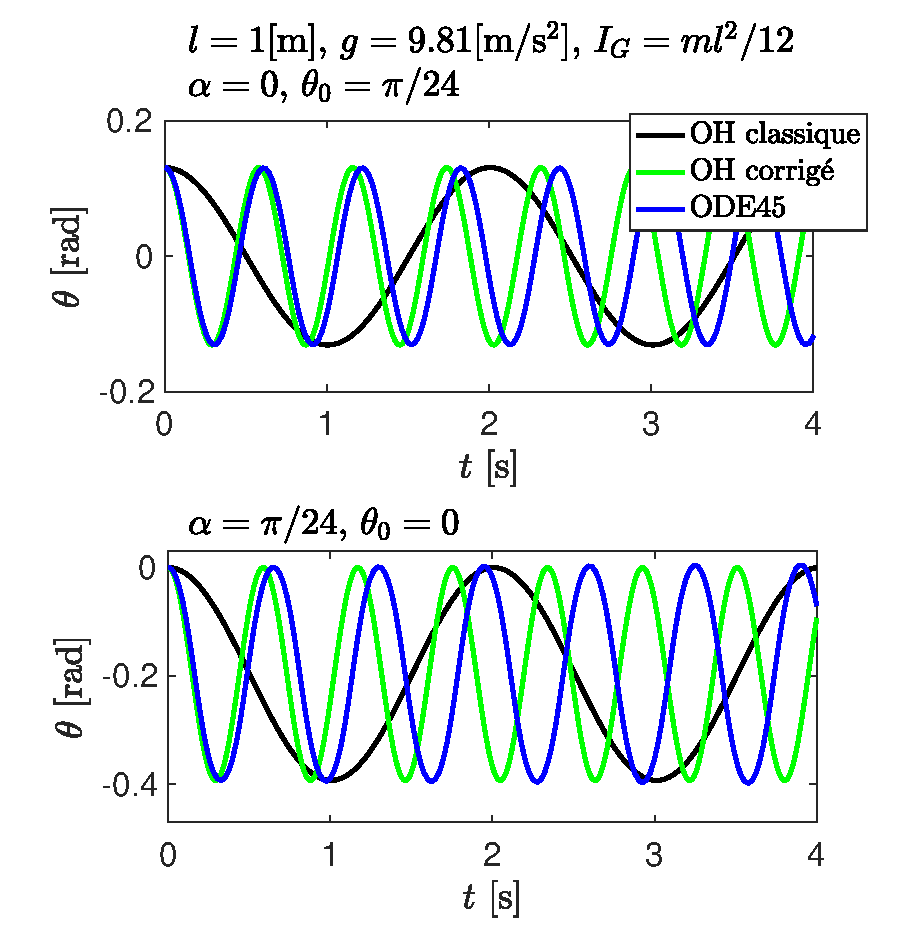
\includegraphics[width=0.95\linewidth]{ExoFig/tyr_solution_petites_oscillations.eps}
  \caption{Petites oscillations autour de l'équilibre.}
    \label{fig:solution_petites_oscillations}
\end{subfigure}%
\begin{subfigure}{.55\textwidth}
  \centering
    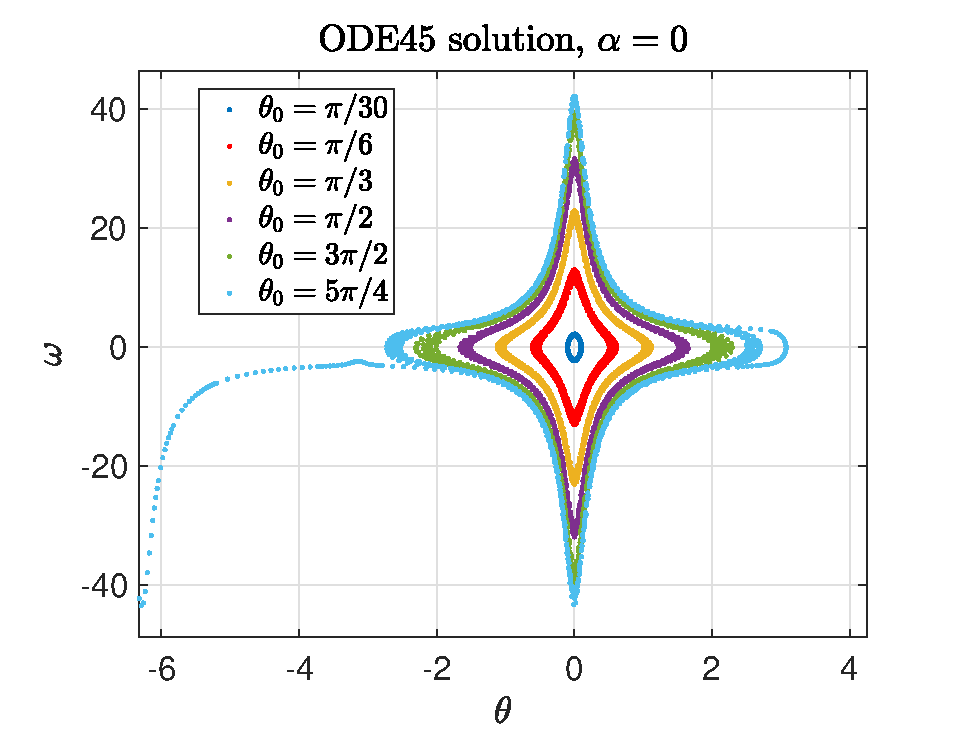
\includegraphics[width=0.95\linewidth]{ExoFig/tyr_solution_espace_de_phase.eps}
  \caption{Trajectoires dans l'espace de phase pour différentes conditions initiales.}
    \label{fig:espace_phase}
\end{subfigure}
\caption{Exemple de trajectoires calculées par \texttt{tyrolienne.m} et ODE45.N.B.: ces résultats utilisent un $\theta$ défini par rapport a la verticale et non par rapport a la perpendiculaire du câble. d'où les oscillations autour de $\theta=-\alpha$.}
\label{fig:test}
\end{figure}

% \begin{figure}
%     \centering
%     \includegraphics[width=0.5\linewidth]{figures/solution_petites_oscillations.eps}
%     \caption{Exemple de trajectoires calculées par \texttt{tyrolienne.m} pour des petites oscillations autour de l'équilibre. N.B.: ces résultats utilisent un $\theta$ défini par rapport a la verticale et non par rapport a la perpendiculaire du câble. d'où les oscillations autour de $\theta=-\alpha$.}
%     \label{fig:solution_petites_oscillations}
% \end{figure}
% \begin{figure}
%     \centering
%     \includegraphics[width=0.5\linewidth]{figures/solution_espace_de_phase.eps}
%     \caption{Exemple de trajectoires dans l'espace de phase calculées par \texttt{tyrolienne.m} différentes conditions initiales. Le solver ODE45 ne conserve plus l'énergie lorsque l'on approche $\theta_0=\pi$ et fait dériver la barre.}
%     \label{fig:espace_phase}
% \end{figure}